% Template for ESA 6th ICATT manuscripts; to be used with:
%          spconf.sty  - LaTeX style file, and
%          IEEEbib.bst - IEEE bibliography style file.
% --------------------------------------------------------------------------
\documentclass{article}
\usepackage{spconf,amsmath,graphicx}
\usepackage{listings}
\usepackage{color}
\usepackage[breaklinks=true, colorlinks=true, pdfstartview=FitV, linkcolor=blue, citecolor=black, urlcolor=black]{hyperref}


% Example definitions.
% --------------------
%\def\x{{\mathbf x}}
%\def\L{{\cal L}}

\definecolor{dkgreen}{rgb}{0,0.6,0}
\definecolor{gray}{rgb}{0.5,0.5,0.5}
\definecolor{mauve}{rgb}{0.58,0,0.82}

\lstdefinestyle{myScalastyle}{
  frame=tb,
  language=scala,
  aboveskip=3mm,
  belowskip=3mm,
  showstringspaces=false,
  columns=flexible,
  basicstyle={\small\ttfamily},
  numbers=none,
  numberstyle=\tiny\color{gray},
  keywordstyle=\color{blue},
  commentstyle=\color{dkgreen},
  stringstyle=\color{mauve},
  frame=single,
  breaklines=true,
  breakatwhitespace=true,
  tabsize=3,
}
\lstset{language=Pascal}

% Title.
% ------
\title{An implementation of SGP4 in non-singular variables \\
              using a functional paradigm}

% Two addresses (uncomment and modify for two-address case).
% ----------------------------------------------------------

\twoauthors{Pablo Pita Leira}{pablo.pita@gmail.com}{Mart\'in Lara%}{mlara0@gmail.com}
\sthanks{Funded by the Ministry of Economic Affairs and Competitiveness of Spain: Projects ESP2013-41634-P and ESP2014-57071-R.}
  }{GRUCACI -- Scientific Computation Group \\ University of La Rioja \\ C/ Luis de Ulloa, s/n. Edificio Vives,  \\
    26004 Logro\~no, Spain}

%

\begin{document}

%\ninept
%
\maketitle
%
\begin{abstract}

A new implementation of the SGP4 algorithm is presented, which allows for choosing different sets of variables in the computation of the periodic corrections. The project is implemented in Scala, a hybrid functional/object oriented programming language running in the Java Virtual Machine that allows for incorporating functional features in the project design.
Validation of the new implementations is made by carrying out different tests based on Vallado's results. Finally, applicability for massive data processing tasks like prediction of orbital collision events and performance are discussed.

\end{abstract}
%
\begin{keywords}
SGP4, Orbital Propagation, Scala, Perturbation theory, non-singular variables
\end{keywords}
%

\section{INTRODUCTION TO SGP4Extensions} \label{sec:intro}

The SGP4 (Simplified General Perturbations 4) orbit propagator is a widely used tool for the fast, short term propagation of earth satellite orbits. The algorithms in which it is based are thoroughly described in the SPACETRACK report \#3 \cite{HootsRoehrich1980}, as well as in Vallado et al.~update \cite{ValladoCrawfordHujsakKelso2006}. Current implementations of SGP4 are based on Brouwer's gravity solution \cite{Brouwer1959} and Lane atmospheric model \cite{Lane1965}, but using Lyddane's modifications for avoiding loss of precision in the evaluation of the periodic corrections \cite{Lyddane1963}, which are, besides, notably simplified for improving evaluation efficiency. Different alternatives in the literature discuss other variable sets, either canonical or not, that can be used in the computation of periodic corrections (see, for instance, \cite{Izsak1963AJ,Aksnes1972,Hoots1981,Lara2015MPE}).
\par

Due to its popularity, there are numerous versions of SGP4 in several programming languages. The most important implementation comes from Vallado \cite{ValladoCrawfordHujsakKelso2006} who has done a comprehensive analysis of the algorithm. Many other versions are derived from his work. The work presented in this paper also derives from Vallado's software. This new implementation, called SGP4Extensions is written in a programming language called Scala. It is hosted in http://github.com/pleira/SGP4Extensions and licensed with an open source Apache Version 2 license.

The SGP4Extensions software differs from Vallado's software in three main points:
\begin{enumerate}
  \item  It is heavily influenced by the functional software paradigm,
  \item  equations have been expressed almost always literally writing the algebraic equations in the code as expressed in the papers
  \item  implementations using other variables and/or extra terms can be easily introduced into the propagation algorithm.
\end{enumerate}
In particular, the usage of Lara's non-singular variables \cite{Lara2015MPE} is optional for all periodic corrections, in this way avoiding the mixture of Lyddane's and polar variables used for the long- and short-period corrections, respectively, in the original implementation.

Besides, SGP4Extensions is designed to provide more options when being used within other algorithms, like those performing space debris conjunction analysis.

In the current version of SGP4Extensions, only extensions around SGP4 are implemented. The deep space algorithm SDP4 is not implemented.

\section{SCALA}
\label{sec:scala}

Scala has been created by Martin Odersky as an hybrid language allowing for architecting software in object oriented and functional paradigms \cite{scala-overview-tech-report}. It is designed with Java compatibility in mind. Users normally compile scala programs to Java byte code that will run in the Java Virtual Machine.

As software complexity increases due to demands like concurrent tasks and parallelism,
there has been a trend in the last years to introduce the functional paradigm where
functions are implemented in a referential transparent way, with no side effects \cite{ChBj}.
No mutable state is kept within the functions. Effects are moved to the outer layers
of the program. All this allows for simpler reasoning about the program which enables
implementing concurrent and parallel solutions more effectively.

The SGP4 algorithm is implemented foremost with the Interpreter Pattern in mind.
There is an intentional
separation of the run time part that has state, like reading/writing to files, called
generally the interpreter, from a pure functional part, the description, which is just
responsible to describe the algorithms that will be applied.
Therefore, mutable state and side effects are avoided in the description part.
The algorithms just return new immutable structures
with the calculations carried out.

\subsection{Spire}
\label{sec:spire}

A scala library called spire is used for providing different efficient numeric types
and their mathematical functions.
The implementation of almost all functions and methods in SGP4Extensions
are parameterized in the numeric types. As example, this function is parameterized
in F which is constraint to have Field operations:

Field is a type in spire that provides for the sum, product and division operation
following associative laws. The algorithm to calculate Lane Coefficients is expressed in Field terms.
There is no problem to call it with types like Double or Reals as the compiler can
convert them to Fields by using Type Classes [{\color{red}provide reference}].

The user has a tradeoff where she can use numeric types with different properties,
like being more exact or carrying its error interval
at the expense of longer computation types.

For testing SGP4Extensions, Double has been used as it is fast and sufficient in SGP4 for almost all cases.
Using an exact numeric type like Real resulted in execution types two orders of magnitude slower.


\subsection{Description of the types used}
\label{sec:typesystem}

Numerous types are used to make clear the data structures and processing
steps involved in this new SGP4 implementation.

Coordinate types and supporting classes for coordinate transformations:
\begin{itemize}
\item SGPElems: classical keplerian elements plus bStar and a julian date)
\item Cartesian: orbital position and velocity in cartesian
\item SpecialPolarNodal: polar nodal coordinates with the inclination instead of the polar component of the angular momentum
\item PolarNodal: \cite{}
\item LaraNonSingular
\item LyddaneElems
\end{itemize}

Models for the corrections like:
\begin{itemize}
\item BrouwerLaneSecularCorrections
\item LyddaneLongPeriodCorrections
\item Lyddane2ndOrderLongPeriodCorrections
\item LaraFirstOrderCorrections
\end{itemize}

Resolution of different Kepler equations because of
different coordinate systems: SimpleKeplerEq, TwoTermsKeplerEq.

[{\color{red}Check that figures are referenced in the final version of the text}]

% // TODO: introduce the different figures with algorithms
% Vectorised image formats like .pdf and .eps are preferred -------------------------------------------------------------------------
\begin{figure}[htb]
  \centering
	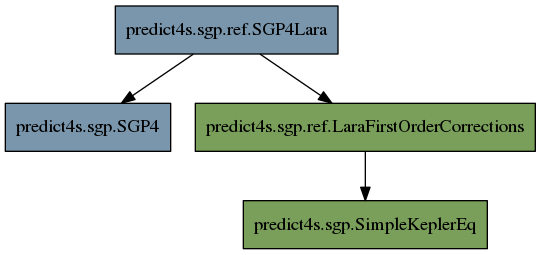
\includegraphics[width=\linewidth]{lara.png}
\label{fig:res}
\caption{SGP4 Algorithm in Lara Non Singular variables}
\end{figure}

\begin{figure*}[htb]
  \centering
	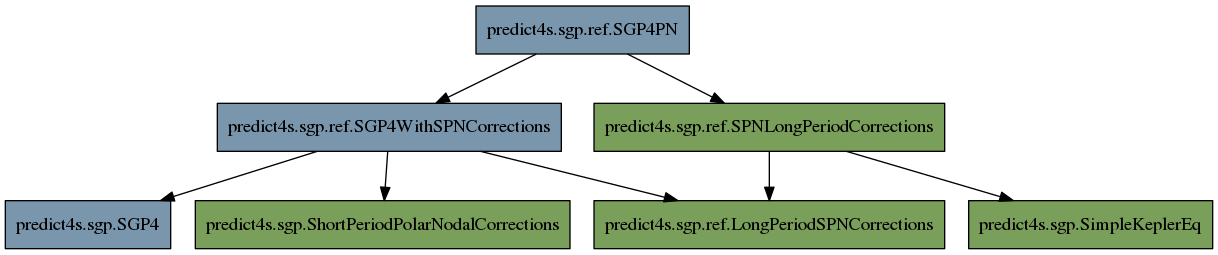
\includegraphics[width=\linewidth]{pn.png}
\caption{SGP4 Algorithm in Polar Nodals}
\end{figure*}

\subsection{Unicode usage}
\label{sec:unicodeusage}

The support in Scala for unicode variables has been used intensively in all Model,
Coordinate and Correnction classes or traits. That allowed to write
the equations in the software similar to those given in the literature, with some
simplifications as no prime or dots for derivatives have been used.

% This method shows the calculation of Lane coefficients of atmospheric drag:

%\begin{lstlisting}%[style=myScalastyle]
%private def calcLaneCoefs[@sp(Double) F : Field](gcoefs : GeoPotentialCoefs[F]) : LaneCoefs[F] = {
%  import gcoefs._
%  val `C1²` = C1*C1
%  LaneCoefs(
%       3*C1/2,
%       D2 + 2*`C1²`,
%       (3*D3 + C1*(12*D2 + 10 * `C1²`))/4,
%       (3*D4 + 12*C1*D3 + 6*D2*D2 + 15*`C1²`*(2*D2+`C1²`))/5)
%}
%\end{lstlisting}

As example, here is the Lyddane 2nd Order Long Period Corrections:
\begin{lstlisting}%[style=myScalastyle]
val δI =   ϵ3 * esinω * c
val δa =   0
val δh = - ϵ3 * ecosω * c/s_
val δC = - ϵ3 * ecosω * esinω * (1/s_ - 2*s_)
val δS =   ϵ3 * s_ - ϵ3*`η²`*s_ - 2*ϵ3*`ecosω²`*s_ + ϵ3*`ecosω²`/s_
val δF =   ϵ3 * s * ecosω * (1 - 2*`η²`/(1+η)) / 2
\end{lstlisting}

\subsection{Optimizations}
\label{sec:optimizations}

All numeric methods use the @specialized compiler feature for the Double numeric type.
The convenient usage of primitive types like Double in generic collections comes with
the cost of boxing/unboxing operations. The compiler
must create wrapper objects for that, an operation called boxing. With @specialized
the compiler will support creating specialized methods or classes for the
declared primitive types that avoid creating the boxing objects.

% // TODO: can we have cache friendly data structures?
% // TODO: can we have primitive type friendly collections (no box/unbox)?



\section{SGP4 ALGORITHM DESCRIPTIONS}
\label{sec:algorithms}

The SGP4 propagator is thoroughly described in the literature \cite{HootsRoehrich1980,ValladoCrawfordHujsakKelso2006}. For completeness, we summarize it here, yet without mentioning anything related to the deep space or atmospheric drag corrections.

% Mi estructura:
% subseccion más importante con la descripción del algoritmo de Vallado
% an~adir subseccion en No Singulares
% si hay sitio, an~adir subsección con Vallado Long y Polares Nodales.
% o estas dos unirlas a una subsección para descartar efectos de haber
% calculado la anomalía verdadera con anterioridad a las correcciones de largo periodo
%
% Tenemos que converger la notación de las ecuaciones en todos los algoritmos
% (Vallado, Vallado Long, Polares Nodales y no singulares).
% Tener las ecuaciones de tal modo que el código en Scala las refleje exactamente
% Eso es posible gracias al soporte de Unicode que ofrece Scala.
% Mencionar en algún sitio que no hay problema con el cálculo de la anomalía.
% la prueba es que Vallado Long y Polares Nodales coinciden a E-7 despues de las
% correcciones de largo periodo.

% Se trata pues de hacer lo siguente en tu artículo en Latex:
%- quitar el código fortran del artículo
%- dejar por tanto las ecuaciones, donde se describen el potencial, las correcciones, las coordenadas usadas ...
%- A~nadir la parte de Vallado Long y de Polares Nodales de tus otros artículos.
%- transformar (si es posible) algunos términos de las ecuaciones para tener la misma notación tanto en Vallado (y demás) como en no singulares:
% * por ejemplo, 1-e*e es en Vallado beta al cuadrado β² y en alguna formula tuya una n larga al cuadrado
% * converger en usar c y s para el coseno/seno de la inclinación (Vallado usa theta en las expresiones del geopotencial)
%   (te parece bien?, pues Hoots/Roerich usan theta en su documento sobre Spacetrack #3)
% * introducir las variables ϵ2 y ϵ3 en las expresiones de Vallado (las hacen más faciles de comparar con las ecuaciones en no singulares o en polares nodales, no te parece?)



First, we recall that Brouwer's gravitational theory relies on the canonical set of Delaunay variables
\begin{itemize} \itemsep0em
\item $\ell=M$: mean anomaly
\item $g=\omega$: argument of the periapsis
\item $h=\Omega$: RAAN (right ascension of the ascending node)
\item $L=\sqrt{\mu\,a}$: Delaunay action, where $\mu$ is the earth gravitational constant and $a$ is the orbit semi-major axis
\item $G=\sqrt{\mu\,p}$: total angular momentum, where $p=a(1-e^2)$ is the orbit parameter (\textit{semilatus rectum}), and $e$ is the orbit eccentricity
\item $H=G\cos{I}$: projection of the angular momentum on the earth's rotation axis, where $I$ is the orbit inclination
\end{itemize}
However, Brouwer's theory finds trouble when evaluating the short-period corrections for the lower eccentricity orbits. The trouble is artificial, and is related to the singularity of Delaunay variables for circular orbits. Hence,
SGP4 implements a different set of elements based on Lyddane's approach which completely avoids that trouble. In particular, the elements used in the computation of short-period corrections are\footnote{The original variables proposed by Lyddane were $a$, $F$, $e\cos\ell$, $e\sin\ell$, $\sin\frac{1}{2}I\cos{h}$, and $\sin\frac{1}{2}I\sin{h}$. }
\[
F=\ell+g+h, \quad C=e\cos\omega, \quad S=e\sin\omega, \quad a, \quad I, \quad h.
\]

\subsection{Standard implementation of SGP4} \label{sec:vallado}

\subsubsection{Initialization and secular corrections}
The code, starts from the initial mean elements at epoch $(I_0,\Omega_0,e_0,\omega_0,M_0,n_0)$, where $n$ stands for mean motion, which should be obtained from the so called two line elements, or TLEs.\footnote{The mean motion read from a TLE needs to be converted from Kozai's definition to Brouwer's secular one.} From them, Delaunay elements at epoch $(\ell_0'',g_0'', h_0'',L_0'',G_0'',H_0'')$ are obtained from their definition. The double prime notation is used for ``secular'' elements. In fact, the Delaunay actions, viz.~$L$, $G$, and $H$, are never computed in SGP4, which uses $n=\mu^2/L^3$, $e=\sqrt{1-G^2/L^2}$, and $I=\arccos(H/G)$, instead.

From these initial elements, Brouwer's theory provides the secular frequencies $\dot\ell''$, $\dot{g}''$, and $\dot{h}''$, due to the earth's gravitational potential, where the overdot means time derivative. Each of these frequencies is a function of $(n_0,e_0,I_0)$, and remain constant for the evaluation of the theory at different dates. Besides, the initialization process provides a series of coefficients needed to apply drag secular corrections as computed from Lane's theory \cite{Lane1965}.
\par

The code works with internal units of length $\mathrm{LU}$ (units of earth's radius $R_\oplus$ in km) and time $\mathrm{TU}$ (units of the orbit's period in min) such that $\mu=1\,\mathrm{LU^3/TU^2}$ in internal units. Besides, the expansion of the gravitational potential in SGP4 is limited to the (unnormalized) zonal harmonics $J_2$, $J_3$, and $J_4$. This selection of units helps in optimizing the code, but it is irrelevant for the description of the algorithms. Therefore, following descriptions include explicitly both the earth's gravitational parameter as well as the earth's equatorial radius.

The next step is to update the secular elements at epoch to the desired date given by the time $t$.

Brouwer's gravitational corrections are applied first
\[
\ell''_j=M_0+\dot\ell''\,t, \quad g''_j=\omega_0+\dot{g}''\,t, \quad h''_j=\Omega_0+\dot{h}''\,t, %\qquad L''_j=L_0, \quad G''_j=G_0, \quad H''=H_0
\]
where the subindex $j$ stands for gravitational effects only. Besides, corrections due to the atmospheric drag, which are not discussed in the paper, are incorporated at this stage.
%\begin{eqnarray*}
%\delta_h &=&  ({21}/{4})J_2({R_\oplus^2}/{p_0^2})\beta_0^2\cos{I}_0\,(n_0C_1t^2) % {\color{red}\quad\verb.units?.}
%\\
%\delta_L &=&  (L''/L_0)=1 - C_1t - D_2t^2 - D_3t^3 - D_4t^4 \\
%\delta_e &=&  (e_0''-e'')=B^*C_4t \\
%\delta_\ell &=&  (\ell''-\ell_j'')/n_0''=T_2\,t^2+T_3\,t^3+T_4\,t^4+T_5\,t^5
%\end{eqnarray*}
%where $\beta_0^2=1-e_0^2$, and $p=a_0\beta_0^2$.
%The necessary constants and coefficients $C_k$, $D_k$, $T_k$, $B^*$, etc.~have been evaluated at the initialization stage.
%Then compute the secular elements (not exactly secular: they mix long-period terms from drag)
%\begin{eqnarray*}
%\ell'' &=&  \ell''_j+n_0''\delta_\ell + {\color{red}\Delta_\ell} \\
%g'' &=&  g''_j - {\color{red}\Delta_\ell} \\
%h'' &=&  h''_j+\delta_h \\
%a'' &=& {L''^2}/{\mu}=({L_0^2}/{\mu})\,({L''}/{L_0})^2=a_0\,\delta_L^2=({\mu}/{n_0^2})^{1/3}\delta_L^2 \\
%e'' &=& e''_0-\delta_e - B^*C_5\left[\sin(\ell_j''+{\color{red}\Delta_\ell})-\sin\ell_0''\right]\\
%I'' &=&  I''_0 .
%\end{eqnarray*}
%where ${\color{red}\Delta_\ell}$ is a long-period correction (see \cite{HootsRoehrich1980}, p.~41).

After that, we obtain the set of secular elements
\[
(\ell'',g'',h'',a'',e'',I'').
\]
The secular mean motion $n''=(\mu/a''^3)^{1/2}$ is also computed.

\subsubsection{Geopotential periodic corrections} \label{s:SGP4lp}

% {\color{red}Remind that I do not deal with the deep space secular corrections}

Brouwer long-period gravitational corrections are reformulated in Lyddane's variables. At the precision of SGP4, there are only corrections for $F$ and $S$. At the precision of SGP4, $C'= C''$, $a'=a''$, $h'=h''$, $I'=I''$, and
\begin{eqnarray*}
F' &=& (\ell''+g''+h'')-\frac{J_3}{4J_2}\frac{R_\oplus}{p''}C''\frac{3+5\cos{I}''}{1+\cos{I}''}\sin{I}'' \\
S' &=&  e''\sin{g}'' -\frac{J_3}{2J_2}\frac{R_\oplus}{p''}\sin{I}''
\end{eqnarray*}
where $C''=e''\cos{g}''$, $p''=a''(1-e''^2)$. The single prime notation means that Lyddane elements include long-period effects. Note that $n'=n''$.



It follows a change from Lyddane's to polar variables
\[
(r,\theta,R=\dot{r},\Theta=r^2\dot\theta)\longrightarrow(F,C,S,a).
\]
To do that, first the Kepler equation
\[
U\equiv{F'-h'}=\Psi+S'\cos\Psi-C'\sin\Psi,
\]
is solved to compute $\Psi=E'+g'$, where $E$ is the eccentric anomaly. Newton-Raphson iterations start from $\Psi_0=U$.

Next $g'$ and $e'$ are solved from $C'=e'\cos{g'}$, $S'=e'\sin{g}'$. Then, compute $E'=\Psi-g'$, $L'=\sqrt{\mu{a}'}$, and $\beta'=\sqrt{1-e'^2}$. It follows the usual transformation
\begin{eqnarray} \label{utor}
r' &=& a'(1-e'\cos{E}') \\
R' &=& (L'/r')e'\sin{E}' \\
\Theta' &=& L'\beta' \\
\theta' &=& f'+g'
\end{eqnarray}
where the true anomaly is obtained without ambiguity from
\begin{equation} \label{utof}
\sin{f}'=(a'/r')\beta'\sin{E}',\quad \cos{f}'=(a'/r')(\cos{E}'-e').
\end{equation}
Note that, SGP4 computes the correction to $r\dot\theta=\Theta/r$ instead of that for the polar variable $\Theta$.


% \subsubsection{Short-period gravitational corrections}

Then, compute $p'=a'\beta'^2$, $c'=\cos{I}'$, $s'=\sin{I}'$, and $\epsilon=\frac{1}{2}J_2(R_\oplus/p')^2$, to obtain the short-period corrections
\begin{eqnarray*}
r-r' &=& r'\epsilon\left[\frac{p'}{r'}\frac{1}{2}(1-c'^2)\cos2\theta'-\frac{3}{2}\beta'(3c'^2-1)\right] \\
\theta-\theta' &=& -\epsilon\frac{1}{4}(7c'^2-1)\sin{2\theta'} \\
h-h' &=& \frac{3}{2}\epsilon c'\cos\theta' \\
R-R' &=& -p'n'\epsilon(1-c'^2)\sin2\theta' \\
I-I' &=& \frac{3}{2}\epsilon c'\,s'\cos2\theta' \\
\frac{\Theta}{r}-\frac{\Theta'}{r'} &=& \frac{\Theta'}{r'}
\epsilon\frac{r'}{p'}\left[\left(1-c'^2\right)\cos2\theta'+\frac{3}{2}\left(3c'^2-1\right)\right]
\end{eqnarray*}


Finally, the state vector is computed from the standard transformation from Cartesian to polar-nodal variables
\[ %\begin{equation} \label{Kepler:Whittaker}
\left(\begin{array}{cc} x & \dot{x} \\ y & \dot{y} \\ z & \dot{z} \end{array}\right)=
R_3(-h)\,{R}_1(-I)\,{R}_3(-\theta)\,\left(\begin{array}{cc} r & R \\ 0 & \Theta/r \\ 0 & 0 \end{array}\right)
\] %\end{equation}
where $R_1$ and $R_3$ are the usual rotation matrices about the $x$ and $z$ axes, respectively


\subsection{Lara's algorithm in non-singular variables} \label{sec:lara}

A straightforward alternative to the SGP4 implementation is to proceed in Lara's non-singular variables \cite{Lara2015MPE} both for the long- and short-period gravitational corrections. The modifications to the SGP4 algorithm start from Section \ref{s:SGP4lp} as follows.

Now, Kepler equation $\ell''=E''-e''\sin{E}''$ must be solved first to compute first the (secular) eccentric anomaly, and then the (secular) true anomaly
\[
f''=2\arctan\left(\sqrt{\frac{1+e''}{1-e''}}\tan\frac{E''}{2}\right).
\]
\par

Next, Delaunay variables are transformed to polar variables using the same equations as Eqs.~(\ref{utor})--(\ref{utof}) but now with double prime variables, which in turn are transformed to Lara's non-singular variables
%$\psi=\theta+h$, $\xi=\sin{I}\sin\theta$, $\chi=\sin{I}\cos\theta$, $r$, $R$, $\Theta$
\[
\psi=\theta+h,\quad \xi=\sin{I}\sin\theta,\quad \chi=\sin{I}\cos\theta,\quad r,\; R,\; \Theta.
\]

Then, apply the long-period corrections (simplified according SGP4 criteria)
\begin{eqnarray*} \label{dyns}
\delta\psi &=& 2\epsilon_3\,\chi
\\  \label{dxins}
\delta\xi &=&  % 2\epsilon_3\chi^2=
\chi\,\delta\psi
\\ \label{dchins}
\delta\chi &=& %-2\epsilon_3\,\chi\,\xi=
-\xi\,\delta\psi
\\ \label{drns}
\delta{r} &=& p\epsilon_3\,\xi,
\\ \label{dRRns}
\delta{R} &=& % ({\Theta}/{p})\,\epsilon_3\,\chi=
(\Theta/r)\,\epsilon_3\,(p/r)\,\chi
\\ \label{dZZns}
\delta\Theta &=& \Theta\epsilon_3\left[\left(\frac{p}{r}-1\right)\xi-\frac{p R}{\Theta}\chi\right].
%\\ \label{dNNns} \color{red}
%\delta{N} &=& 0,
\end{eqnarray*}
where, $\epsilon_3=\frac{1}{2}(J_3/J_2)(R_\oplus/p)$.
\par

It follows the computation of the short-period corrections (simplified according SGP4 criteria)
\begin{eqnarray*}
\Delta\psi &=& -\epsilon_2\frac{1+7c}{1+c}\,\xi\,\chi,
\\
\Delta\xi &=& -\epsilon_2\left(\chi^2-3c^2\right)\xi,
\\[1ex]
\Delta\chi &=& \epsilon_2\left(\xi^2-3c^2\right)\chi,
\\
\Delta{r} &=& % \epsilon_2p\left[(\xi^2-\chi^2)+3(2-3s^2)\right]=
\epsilon_2r\left[(\xi^2-\chi^2)-3(1-3c^2)\right],
\\
\Delta{R} &=& %4\epsilon_2\,(\Theta/p)\xi\,\chi=
4\epsilon_2\,(\Theta/r)\xi\,\chi,
\\
\Delta\Theta &=&  3\epsilon_2\,\Theta(\xi^2-\chi^2),
\end{eqnarray*}
where $c=\cos{I}$, $s=\sin{I}$, and $\epsilon_2=-\frac{1}{4}(R_\oplus/p)^2J_2$.
\par

Finally, the state vector is computed from
\begin{eqnarray*} \label{ns2x}
x &=& r\,(b\cos\psi+q\sin\psi), \\ \label{ns2y}
y &=& r\,(b\sin\psi-q\cos\psi), \\
z &=& r\,\xi, \\
X &=& x\,(R/r) %(b\cos\psi+q\sin\psi)
 - ({\Theta}/{r})\,(q\cos\psi+\tau\sin\psi), \\ \label{ns2Y}
Y &=& y\,(R/r) %(b\sin\psi-q\cos\psi)
 - ({\Theta}/{r})\,(q\sin\psi-\tau\cos\psi), \\  \label{ns2zz}
Z &=& z\,(R/r)+(\Theta/r)\,\chi,
\end{eqnarray*}
where
\[%\begin{equation} \label{tq}
b=1-\frac{\xi^2}{1+c}, \qquad
\tau=1 - \frac{\chi^2}{1 + c}, \qquad
q=\frac{\xi\,\chi}{1+c},
\]%\end{equation}
and $c=H/\Theta$. Remark that $H$ is an integral of the zonal problem and, therefore, its value is always known from given initial conditions $H=H_0''$.



% TODO: should we revise the Short Period Corrections in non-singular variables?
%       objective: better match in the plots

\subsection{True anomaly} \label{sec:trueanomaly}

{\color{red}\dots Pablo \dots}

To verify that the order in which the eccentric anomaly is calculated does not have effect,
two additional algorithms have been done:

Vallado with extra terms for the long period corrections

Polar Nodals variant as in Lara where first solve Kepler Equation and then the Long Period Corrections are calculated in Polar Nodals variables.

%Equations shall be centred in the column and the corresponding number aligned on the right. They shall be referenced using parenthesis, e.g.,~\eqref{eq:ellipse}.

%\begin{equation}
%r=\dfrac{p}{1+e\cos\theta}
%\label{eq:ellipse}
%\end{equation}

%The paper title (on the first page) should begin 1.38 inches (35 mm) from the
%top edge of the page, centered, completely capitalized, and in Times 14-point,
%boldface type.  The authors' name(s) and affiliation(s) appear below the title
%in capital and lower case letters.  Papers with multiple authors and
%affiliations may require two or more lines for this information.

%\section{TYPE-STYLE AND FONTS}
%\label{sec:typestyle}

%To achieve the best rendering, only use Times-Roman font. In addition, this will give
%the proceedings a more uniform look.  Use a font that is no smaller than nine
%point type throughout the paper, including figure captions.

%In nine point type font, capital letters are 2 mm high.  {\bf If you use the
%smallest point size, there should be no more than 3.2 lines/cm (8 lines/inch)
%vertically.}  This is a minimum spacing; 2.75 lines/cm (7 lines/inch) will make
%the paper much more readable.  Larger type sizes require correspondingly larger
%vertical spacing.  Please do not double-space your paper.  TrueType or
%Postscript Type 1 fonts are preferred.

%The first paragraph in each section should not be indented, but all the
%following paragraphs within the section should be indented as these paragraphs
%demonstrate.

\section{SAMPLE TEST CASES}
\label{sec:sampletestcases}


\subsection{Subheadings}
\label{ssec:subhead}

%Subheadings should appear in lower case (initial word capitalized) in
%boldface. They should start at the left margin on a separate line.


\section{VALIDATION}
\label{sec:validation}

The validation of the software has been done by comparing the results with those
of Vallado's original C++ source. The C++ source has been slightly modified in order
to save the cartesian coordinates, the unit vector, the polar nodals coordinates
and the long period corrections into a file. The outputs were collected
for the Near Earth test cases. These outputs have been compared with all the propagation
algorithms in SGP4Extensions.


The SGP4Vallado algorithm in Scala matches the C++ results with maximum differences
of the order of 3E-8 for all test propagations.
When propagating 22312 and 28350, the SGP4Vallado implementation went into error earlier
than the C++ version because of negative value for the eccentricity:
22312  454.2028672 474.2028672
28350  960         1440
For the satellite 28872, propagation with SGP4Vallado ends by minute 50 as Vallado's cpp.


%%%
%%% MAYBE THIS TABLE GETS DISCARDED, or make it smaller
%%%
\begin{table*}[p]
\centering
\caption{NEAR EARTH TLEs used for testing}\vspace{2mm}
\begin{tabular}{|l|l|p{14cm}|}
\hline\hline
Satellite & Category & Comments\\
\hline
00005 & Near Earth & TEME example satellite.\\
06251 &  Near Earth  & Near Earth normal drag case. The perigee of 377.26 km is low, but above the threshold of 220
km for simplified equations, so moderate drag case.\\
22312  & NE/S  & Near Earth with very low perigee (86.98 km) that uses the second branch (perigee < 98 km)
for limiting the ‘s4’ drag coefficient to 20. Propagation beyond approximately 2840 min
should result in error trap (modified eccentricity too low).\\
28057 &  Near Earth  & Near Earth normal drag case but with low eccentricity (0.000 088 4) so certain drag terms are
set to zero to avoid math errors / loss of precision.\\
28350 & NE/S  & Near Earth low perigee (127.20 km) that uses the branch (perigee \textless 156 km) for modifying
the ‘s4’ drag coefficient. Propagation beyond approximately 1460 minutes should result in
error trap (modified eccentricity too low).\\
28872  & NE/S  & Sub-orbital case (perigee 51 km, lost about 50 minutes from epoch) used to test error handling.\\
29141  & Near Earth  & Last stages of decay.\\
29238  & NE/S  & Near Earth with perigee 212.24 km, thus uses simplified drag branch (perigee \textless 220 km) test.\\
\hline\hline
\end{tabular}
\label{tab:res}
\end{table*}


% Figures, tables and equations must be numbered and placed within the designated margins. They may span the two
% columns. Every figure and table must also be captioned.

% If possible, position illustrations at the top of columns, rather than in the middle or at the bottom. Figure~\ref{fig:res} shows how to include images.

% For tables, the example on how they shall be captioned and formatted is provided in Table~\ref{tab:res}.



% To start a new column (but not a new page) and help balance the last-page
% column length use \vfill\pagebreak.
% -------------------------------------------------------------------------


\bibliographystyle{IEEEbib}
\bibliography{refs}

% References should be produced using the bibtex program from suitable
% BiBTeX files (here: refs). The IEEEbib.bst bibliography
% style file from IEEE produces unsorted bibliography list.
% -------------------------------------------------------------------------

\end{document}
